\documentclass{report}
\usepackage[spanish]{babel}
\usepackage[left=2.5cm, right=2.5cm, top=3cm, bottom=3cm]{geometry}
\usepackage{enumerate}
\usepackage{geometry}
\usepackage{graphicx}
\usepackage{booktabs}
\usepackage{tabularx}
\usepackage{enumitem}
\usepackage{amsmath}
\usepackage{amsfonts}
\usepackage{float}   

\geometry{
  top=2cm,  bottom=2cm,  left=1.5cm,  right=1.5cm
}

\setlength{\parindent}{0pt}

\begin{document}

    \begin{titlepage}
        \centering
        {\bfseries\LARGE Facultad de Matemática y Computación \par}
        \vspace*{1cm}
        {\scshape\Large Base de Datos II \par}
        \vspace*{3cm}
        {\scshape\Huge Diseño de la base de datos \par}
        \vspace*{1cm}
        {\LARGE \textbf{Tema: Gestión de campeonatos de beisbol} }
        \vfill
        {\bfseries\LARGE Integrantes: \par}
        {\Large Ariadna Vel\'azquez Rey  C311 \par} 
        {\Large L\'ia L\'opez Rosales  C312 \par} 
        {\Large Carlos Daniel Largacha Leal  C312 \par} 
        {\Large Gabriel Andr\'es Pla Lasa  C311 \par} 
        {\Large Raidel Miguel Cabellud Lizaso C311 \par} 
        \vfill
    \end{titlepage}


    \section*{Introducción}

    En este informe se presenta y justifica el diseño de la base de datos a utilizar en el proyecto `` Gestión de 
    campeonatos de beisbol '', para ello se mostrará el Modelo Conceptual (MERX) realizado por el equipo de 
    desarrollo, así como el Modelo Relacional y una justificación del mismo. Además se mencionarán los 
    requerimientos que presenta el proyecto para un mayor entendimiento de la organización de la base de datos.

    \section*{Requerimientos}
    Tras el análisis de la orientación del proyecto y la posterior consulta con algunos de los clientes, se llegó
    a determinar que los requerimientos son:

    \subsection*{Requerimientos Funcionales}
    \begin{enumerate}
        \item Registrar datos por el administrador mediante formularios.
        \item Generar modelos tabulares y gr\'aficos.
        \item Gestionar los roles de la base de dato: usuarios especiales (administrador), los directores técnicos y 
        los usuarios normales (periodistas).
        \item Presentar diferentes vistas para los distintos tipos de roles.
        \item Generar formularios para ingresar los datos a la base de datos por parte del administrador.
        \item Tener un formulario para el director técnico que le permita realizar los cambios en la alineación.
        \item Mostrar un formulario con opciones de filtrado y solicitudes para la generaci\'on de los reportes.
        \item Obtener nombres de equipos ganadores y directores técnicos en series nacionales por temporada.
        \item Obtener nombres y posiciones de jugadores del equipo "Todos Estrellas y su efectividad por serie.
        \item Obtener series con mayor y menor cantidad de juegos celebrados.
        \item Listar equipos en primer y último lugar por serie, clasificados por tipo y orden cronológico.
        \item Obtener el total de juegos ganados por un lanzador y su promedio de carreras limpias permitidas.
        \item Modificar la posición de un jugador en la alineación inicial de un juego específico.
        \item Obtener estadísticas de un jugador.
        \item Exportar reportes a formato PDF, con soporte para la agregación de otros formatos.
    \end{enumerate}

    \subsection*{Requerimientos No Funcionales}

    \subsubsection*{Usabilidad}
    \begin{itemize}
        \item Se espera que la interfaz sea capaz de mostrar gráficas.
        \item Se espera un sistema visual de filtrado para seleccionar qué datos mostrar en los reportes.
    \end{itemize}

    \subsubsection*{Seguridad}
    \begin{itemize}
        \item Todos los datos personales y críticos deben ser encriptados en tránsito y en almacenamiento.
        \item La autenticación y autorización deben ser seguras, asegurando que solo los usuarios autorizados tengan 
        acceso a funcionalidades específicas.
    \end{itemize}

    \subsubsection*{Portabilidad y Compatibilidad}
    \begin{itemize}
        \item El diseño de la interfaz se espera que sea ajustable al tamaño de los distintos dispositivos en los que 
        puede abrirse el sitio web.
        \item Debe ser compatible con los navegadores más utilizados, asegurando que las interfaces web sean 
        responsivas y adaptativas.
    \end{itemize}

    \subsubsection*{Rendimiento}
    \begin{itemize}
        \item El sistema debe ser capaz de manejar múltiples solicitudes simultáneamente sin una degradación 
        significativa en el tiempo de respuesta.
    \end{itemize}

    \subsubsection*{Escalabilidad}
    \begin{itemize}
        \item La arquitectura debe permitir la escalabilidad horizontal y vertical. Esto significa que se debe poder 
        agregar más recursos (como servidores adicionales) para manejar un mayor número de usuarios o datos sin 
        necesidad de reestructurar significativamente el sistema.
    \end{itemize}

    \subsubsection*{Mantenibilidad}
    \begin{itemize}
        \item El sistema debe estar desarrollado con buenas prácticas de programación, como la documentación adecuada 
        (docstring) y código modular.
    \end{itemize}

    \subsubsection*{Extensibilidad}
    \begin{itemize}
        \item La arquitectura del sistema debe ser flexible para permitir la adición de nuevas funcionalidades sin 
        necesidad de grandes modificaciones en el código base.
    \end{itemize}

    \subsubsection*{Almacenamiento, importación y exportación de datos}
    \begin{itemize}
        \item El software deberá de almacenar todos los datos en una base de datos SQL.
        \item El software deberá ser capaz de convertir los reportes solicitados a documentos PDF.
    \end{itemize}

    \section*{Restricciones de Integridad}

    Para garantizar la consistencia, precisión y confiabilidad de los datos en el sistema de gestión de campeonatos 
    de béisbol, se han definido diversas restricciones de integridad. Estas restricciones aseguran que las 
    relaciones entre peloteros, equipos, series y juegos sean válidas y que los datos almacenados cumplan con las 
    reglas del negocio. Se clasifican en tres categorías principales: restricciones de integridad referencial, que 
    mantienen la coherencia entre tablas relacionadas; restricciones de dominio, que limitan los valores permitidos 
    para ciertos atributos; y restricciones específicas del negocio, que reflejan reglas operativas propias del 
    sistema.

    \subsection*{Integridad Referencial}
    \begin{itemize}
        \item \textbf{Relación entre peloteros y equipos:} Un pelotero pertenece a un equipo por serie. 
        \begin{itemize}
            \item Clave foránea: \texttt{Equipo\_ID} en la tabla de peloteros debe referenciar la clave primaria de 
            la tabla de equipos.
        \end{itemize}

        \item \textbf{Relación entre equipos y series:} Un equipo está asociado a una serie específica. 
        \begin{itemize}
            \item Clave foránea: \texttt{Serie\_ID} en la tabla de equipos debe referenciar la clave primaria de la 
            tabla de series.
        \end{itemize}

        \item \textbf{Relación entre juegos y series:} Cada juego pertenece a una serie única.
        \begin{itemize}
            \item Clave foránea: \texttt{Serie\_ID} en la tabla de juegos debe referenciar la clave primaria de la 
            tabla de series.
        \end{itemize}

        \item \textbf{Relación entre alineaciones y juegos:} Cada alineación pertenece a un juego y un equipo 
        específicos.
        \begin{itemize}
            \item Claves foráneas: \texttt{Juego\_ID} y \texttt{Equipo\_ID} en la tabla de alineaciones deben 
            referenciar las claves primarias de las tablas de juegos y equipos, respectivamente.
        \end{itemize}

        \item \textbf{Relación entre lanzadores y juegos:} Los lanzadores registrados deben ser peloteros válidos 
        que jugaron en el juego.
        \begin{itemize}
            \item Clave foránea: \texttt{Pelotero\_ID} en la tabla de lanzadores debe referenciar la clave primaria 
            de la tabla de peloteros.
        \end{itemize}
    \end{itemize}

    \subsection*{Integridad de Dominio}
    \begin{itemize}
        \item \textbf{Dominio para fechas:} 
        \begin{align*}
            \texttt{FechaInicio} < \texttt{FechaFin}
        \end{align*}

        \item \textbf{Dominio para estadísticas:} 
        \begin{align*}
            \texttt{JuegosGanados} \geq 0, \hspace*{0.9cm} \texttt{JuegosPerdidos} \geq 0, \hspace*{0.9cm} \texttt{PromedioCarreras} \geq 0
        \end{align*}

        \item \textbf{Dominio para posiciones:} Los valores de las posiciones deben estar restringidos a:
        \begin{align*}
            \{\texttt{pitcher, catcher, baseman, outfielder, shortstop, etc.}\}
        \end{align*}

        \item \textbf{Dominio para atributos específicos:} 
        \begin{align*}
            \texttt{ManoDominante} \in \{\texttt{derecha, izquierda}\}
        \end{align*}
    \end{itemize}

    \subsection*{Restricciones Específicas del Negocio}
    \begin{itemize}
        \item \textbf{Unicidad de pelotero por serie:} Un pelotero no puede pertenecer a más de un equipo dentro de 
        la misma serie.
        \begin{align*}
            \texttt{UNIQUE(Pelotero\_ID, Serie\_ID)}
        \end{align*}

        \item \textbf{Resultados de juegos:} En un juego deben registrarse un equipo ganador y uno perdedor, y no 
        pueden ser el mismo.
        \begin{align*}
            \texttt{Ganador\_ID} \neq \texttt{Perdedor\_ID}
        \end{align*}

        \item \textbf{Alineación única por juego y equipo:} Un jugador no puede estar en más de una posición en la 
        alineación inicial de un equipo durante un juego específico.
        \begin{align*}
            \texttt{UNIQUE(Juego\_ID, Equipo\_ID, Pelotero\_ID)}
        \end{align*}

        \item \textbf{Relación entre estadísticas y jugadores:} Si un jugador es registrado como lanzador 
        (\texttt{Pitch = True}), deben incluirse sus estadísticas específicas.
        \begin{align*}
            \texttt{JuegosGanados}, \texttt{JuegosPerdidos}, \texttt{PromedioCarreras}
        \end{align*}

        \item \textbf{Jugador estrella:} Los jugadores estrella deben seleccionarse al final de cada serie y no 
        duplicarse para una misma posición en la misma serie.
    \end{itemize}


    \newpage

    \section*{Modelo Conceptual}

    En la \textit{Figura 1} se encuentra el gráfico del MERX que se utilizará como base en el diseño de la base de 
    datos.

    \begin{figure}[H] 
        \centering
        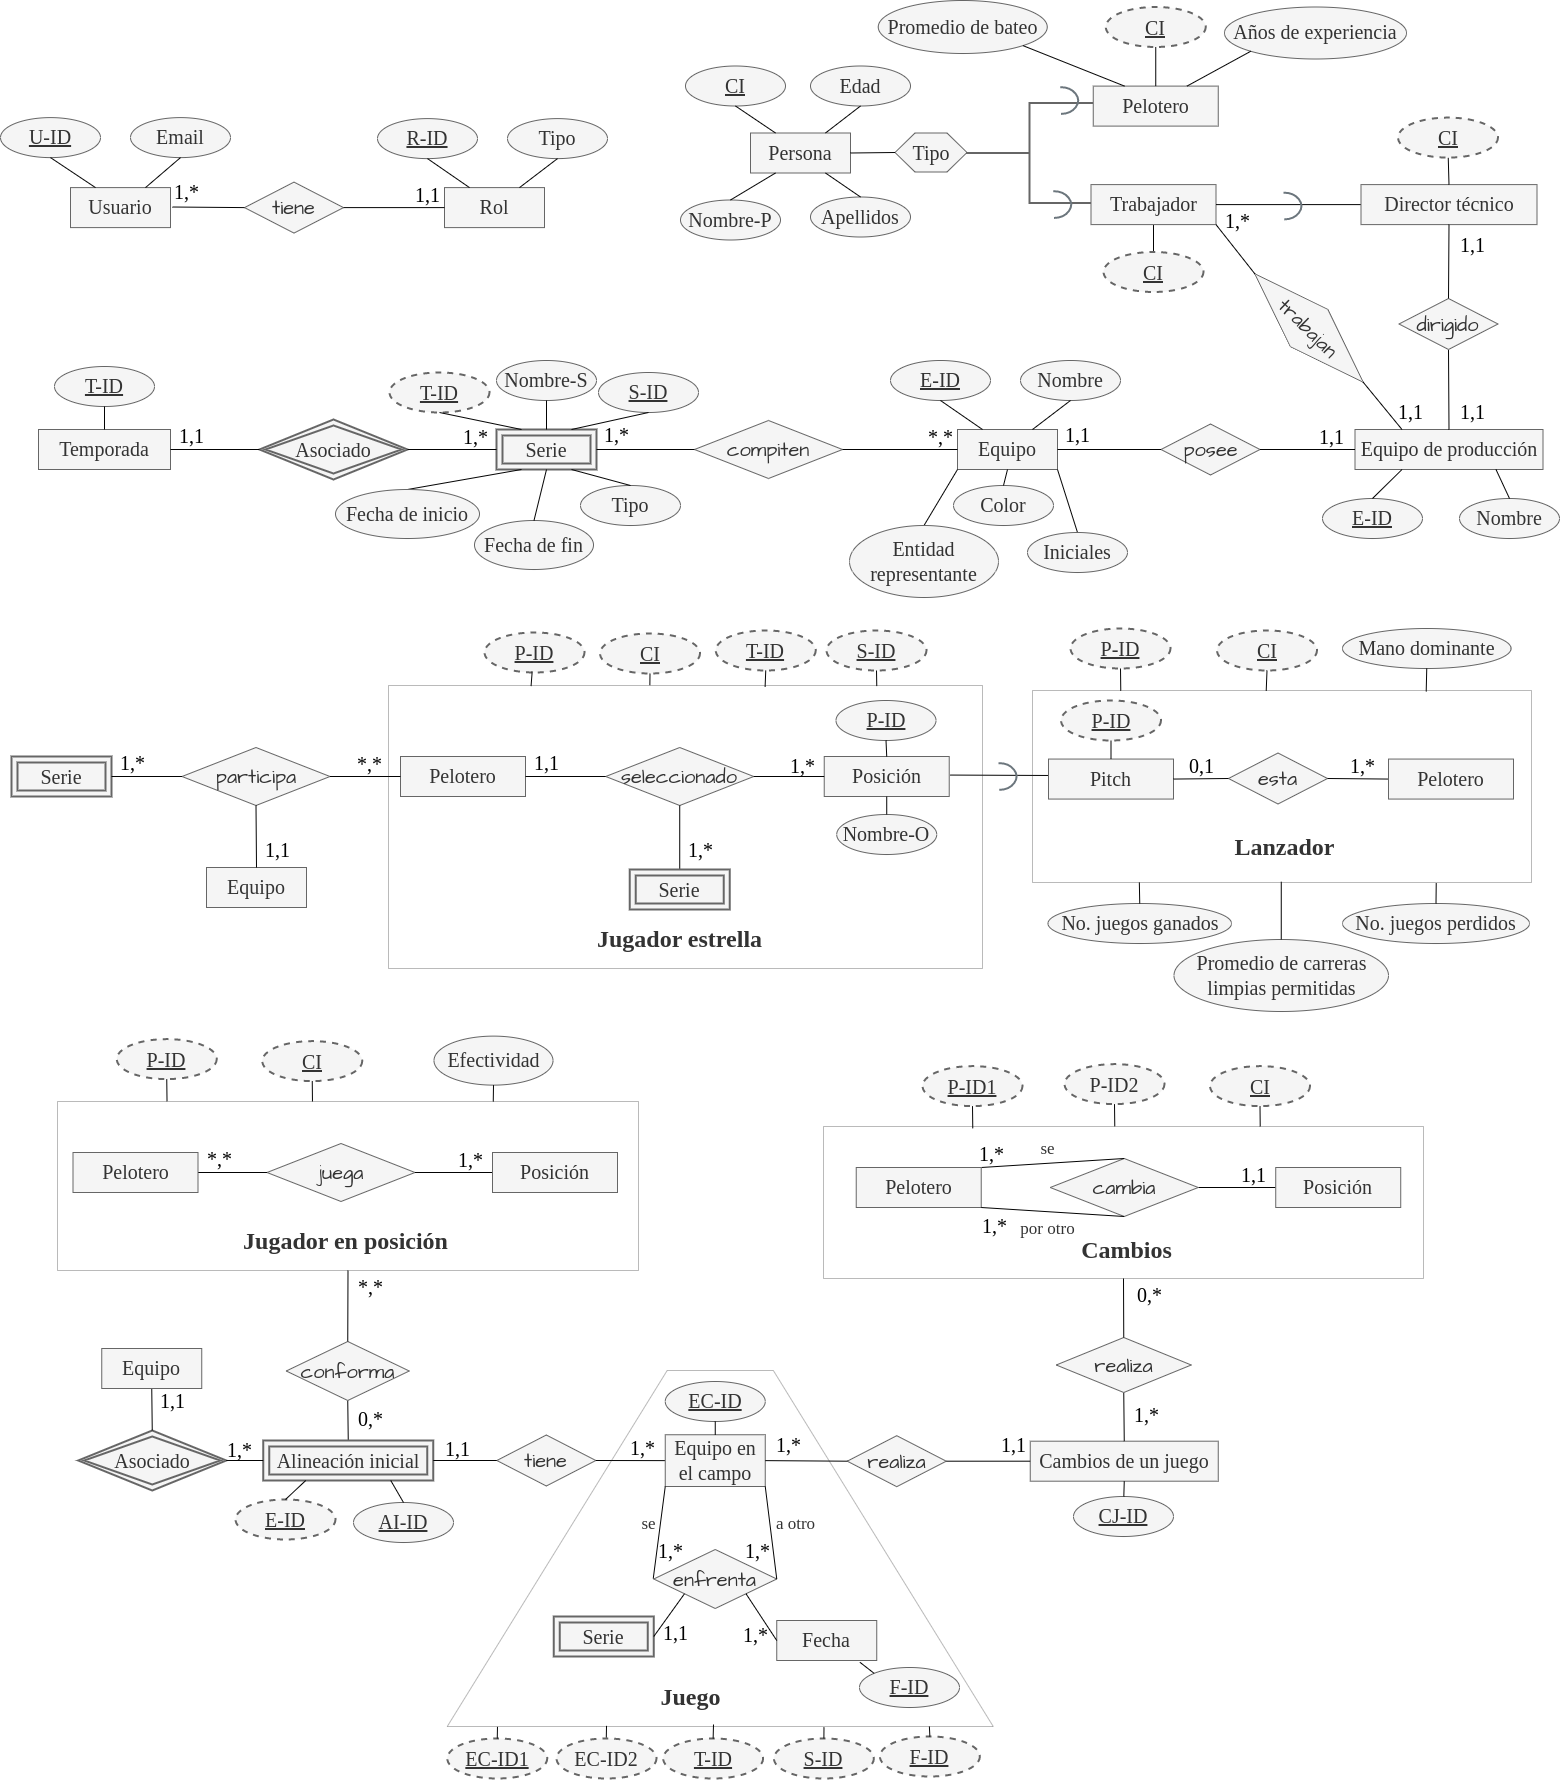
\includegraphics[scale=0.33, keepaspectratio]{baseball_MERX.png}
        \caption{MERX de la Gestión de campeonatos de béisbol}
    \end{figure}

    \newpage

    \section*{Modelo Relacional}

    Para capturar la estructura conceptual del sistema de gestión de campeonatos de béisbol se utilizó MERX y a 
    partir del él, se identificaron las dependencias funcionales que describen cómo los atributos de cada entidad 
    y sus relaciones están determinados por sus claves primarias.Estas dependencias funcionales permitirán 
    establecer la base para normalizar el diseño, asegurando un modelo lógico consistente y alineado con las 
    necesidades del sistema. \\

    En la siguiente tabla se muestran el universo y las dependencias funcionales sacadas a partir del MERX mostrado 
    anteriormete. \newline 

    %\vspace*{0.5cm}
    \begin{tabularx}{\textwidth}{|X|}
        \toprule
        \hfil $\textbf{R(U, F)}$ \\
        \midrule
        \vspace*{0.01cm}
        $U = \{ $ NombreE, Tipo, P-ID, Años de experiencia, CI, Efectividad, Entidad representante, NombreP, Fecha 
        de fin, Email, Edad, E-ID, S-ID, Fecha de inicio, EC-ID, No juegos ganados, EC-ID 2, Pitch, BP-ID, EP-ID, 
        Promedio de bateo, AI-ID, T-ID, Color, F-ID, Promedio carreras, DT-ID, NombreEP, No juegos perdidos, 
        NombreTS, Apellidos, Iniciales, W-ID, NombrePos, BP-ID 2, R-ID, U-ID, Mano dominante, M-ID, E-ID 2, 
        Marcador Ganador, Marcador Perdedor $\} $ 
        \vspace*{0.15cm} \\
        \midrule
        \vspace*{0.01cm}
        $F = \{$
                U-ID $\rightarrow$ Email \newline
                \hspace*{0.9cm} R-ID $\rightarrow$ Tipo \newline
                \hspace*{0.9cm} CI $\rightarrow$ NombreP,  Edad,  Apellidos \newline
                \hspace*{0.9cm} BP-ID $\rightarrow$ CI \newline
                \hspace*{0.9cm} BP-ID $\rightarrow$ Promedio de bateo,  Años de experiencia \newline
                \hspace*{0.9cm} W-ID $\rightarrow$ CI \newline
                \hspace*{0.9cm} W-ID $\rightarrow$ DT-ID \newline
                \hspace*{0.9cm} DT-ID $\rightarrow$ W-ID \newline
                \hspace*{0.9cm} EP-ID $\rightarrow$ NombreEP \newline
                \hspace*{0.9cm} E-ID $\rightarrow$ NombreE,  Color,  Entidad representante,  Iniciales \newline
                \hspace*{0.9cm} E-ID,  AI-ID $\rightarrow$ E-ID,  AI-ID \newline
                \hspace*{0.9cm} T-ID,  S-ID $\rightarrow$ Nombre,  Tipo,  Fecha de inicio,  Fecha de fin \newline
                \hspace*{0.9cm} P-ID $\rightarrow$ NombrePos \newline
                \hspace*{0.9cm} P-ID $\rightarrow$ Pitch \newline
                \hspace*{0.9cm} Pitch $\rightarrow$ P-ID \newline
                \hspace*{0.9cm} CJ-ID $\rightarrow$ CJ-ID \newline
                \hspace*{0.9cm} U-ID $\rightarrow$ R-ID \newline
                \hspace*{0.9cm} W-ID $\rightarrow$ EP-ID \newline
                \hspace*{0.9cm} DT-ID $\rightarrow$ EP-ID \newline
                \hspace*{0.9cm} EP-ID $\rightarrow$ DT-ID \newline
                \hspace*{0.9cm} EP-ID $\rightarrow$ E-ID \newline
                \hspace*{0.9cm} E-ID $\rightarrow$ EP-ID \newline
                \hspace*{0.9cm} T-ID,  S-ID,  E-ID $\rightarrow$ T-ID,  S-ID,  E-ID \newline
                \hspace*{0.9cm} T-ID,  S-ID,  BP-ID $\rightarrow$ E-ID \newline
                \hspace*{0.9cm} T-ID,  S-ID,  P-ID $\rightarrow$ BP-ID \newline
                \hspace*{0.9cm} BP-ID,  Pitch $\rightarrow$ Mano dominante,  No juegos ganados,  No juegos perdidos,  Promedio carreras \newline
                \hspace*{0.9cm} BP-ID,  P-ID $\rightarrow$ Efectividad \newline
                \hspace*{0.9cm} E-ID,  AI-ID,  BP-ID,  P-ID $\rightarrow$ E-ID,  AI-ID,  BP-ID,  P-ID \newline
                \hspace*{0.9cm} EC-ID $\rightarrow$ E-ID,  AI-ID \newline
                \hspace*{0.9cm} BP-ID,  F-ID $\rightarrow$ BP-ID 2,  P-ID,  E-ID \newline
                \hspace*{0.9cm} BP-ID,  F-ID $\rightarrow$ EC-ID \newline
                \hspace*{0.9cm} EC-ID,  F-ID $\rightarrow$ EC-ID 2,  T-ID,  S-ID, M-ID \newline 
                \hspace*{0.9cm} M-ID $\rightarrow$ E-ID, E-ID 2, Marcador Ganador , Marcador Perdedor \newline       
        $\} $
        \vspace*{0.15cm} \\    
        \bottomrule
    \end{tabularx}

    \vspace*{0.5cm}

    En la siguiente tabla se muestran los resultados de aplicar el algoritmo del cubrimiento mínimo a partir de las 
    dependencias funcionales expuestas.

    \begin{tabularx}{\textwidth}{|X|X|X|}
        \toprule
        \hfil F ' & \hfil F ' '  & \hfil F ' ' '  \\
        \midrule
        U-ID $\rightarrow$ Email \newline 
        R-ID $\rightarrow$ Tipo \newline 
        CI $\rightarrow$ NombreP \newline 
        CI $\rightarrow$ Edad \newline 
        CI $\rightarrow$ Apellidos \newline 
        BP-ID $\rightarrow$ CI \newline 
        BP-ID $\rightarrow$ Promedio de bateo \newline 
        BP-ID $\rightarrow$ Años de experiencia \newline 
        W-ID $\rightarrow$ CI \newline 
        W-ID $\rightarrow$ DT-ID \newline 
        DT-ID $\rightarrow$ W-ID \newline 
        EP-ID $\rightarrow$ NombreEP \newline 
        E-ID $\rightarrow$ NombreE \newline 
        E-ID $\rightarrow$ Color \newline 
        E-ID $\rightarrow$ Entidad representante \newline 
        E-ID $\rightarrow$ Iniciales \newline 
        E-ID, AI-ID $\rightarrow$ E-ID \newline 
        E-ID, AI-ID $\rightarrow$ AI-ID \newline 
        T-ID, S-ID $\rightarrow$ NombreTS \newline 
        T-ID, S-ID $\rightarrow$ Tipo \newline 
        T-ID, S-ID $\rightarrow$ Fecha de inicio \newline 
        T-ID, S-ID $\rightarrow$ Fecha de fin \newline 
        P-ID $\rightarrow$ NombrePos \newline 
        P-ID $\rightarrow$ Pitch \newline 
        Pitch $\rightarrow$ P-ID \newline 
        U-ID $\rightarrow$ R-ID \newline 
        W-ID $\rightarrow$ EP-ID \newline 
        DT-ID $\rightarrow$ EP-ID \newline 
        EP-ID $\rightarrow$ DT-ID \newline 
        EP-ID $\rightarrow$ E-ID \newline 
        E-ID $\rightarrow$ EP-ID \newline 
        T-ID, S-ID, E-ID $\rightarrow$ T-ID \newline 
        T-ID, S-ID, E-ID $\rightarrow$ S-ID \newline 
        T-ID, S-ID, E-ID $\rightarrow$ E-ID \newline 
        T-ID, S-ID, BP-ID $\rightarrow$ E-ID \newline 
        T-ID, S-ID, P-ID $\rightarrow$ BP-ID \newline 
        BP-ID, Pitch $\rightarrow$ Mano dominante \newline 
        BP-ID, Pitch $\rightarrow$ No juegos ganados \newline 
        BP-ID, Pitch $\rightarrow$ No juegos perdidos \newline 
        BP-ID, Pitch $\rightarrow$ Promedio carreras \newline 
        BP-ID, P-ID $\rightarrow$ Efectividad \newline 
        E-ID, AI-ID, BP-ID, P-ID $\rightarrow$ E-ID \newline 
        E-ID, AI-ID, BP-ID, P-ID $\rightarrow$ AI-ID \newline 
        E-ID, AI-ID, BP-ID, P-ID $\rightarrow$ BP-ID \newline 
        E-ID, AI-ID, BP-ID, P-ID $\rightarrow$ P-ID \newline 
        EC-ID $\rightarrow$ E-ID \newline 
        EC-ID $\rightarrow$ AI-ID \newline 
        BP-ID, F-ID $\rightarrow$ BP-ID 2 \newline 
        BP-ID, F-ID $\rightarrow$ P-ID \newline 
        BP-ID, F-ID $\rightarrow$ E-ID \newline 
        BP-ID, F-ID $\rightarrow$ EC-ID \newline 
        EC-ID, F-ID $\rightarrow$ EC-ID 2 \newline 
        EC-ID, F-ID $\rightarrow$ T-ID \newline 
        EC-ID, F-ID $\rightarrow$ S-ID \newline
        EC-ID, F-ID $\rightarrow$ M-ID \newline 
        M-ID $\rightarrow$ E-ID \newline 
        M-ID $\rightarrow$ E-ID 2 \newline 
        M-ID $\rightarrow$ Marcador Ganador \newline 
        M-ID $\rightarrow$ Marcador Perdedor & 

        U-ID $\rightarrow$ Email \newline 
        R-ID $\rightarrow$ Tipo \newline 
        CI $\rightarrow$ NombreP \newline 
        CI $\rightarrow$ Edad \newline 
        CI $\rightarrow$ Apellidos \newline 
        BP-ID $\rightarrow$ CI \newline 
        BP-ID $\rightarrow$ Promedio de bateo \newline 
        BP-ID $\rightarrow$ Años de experiencia \newline 
        W-ID $\rightarrow$ CI \newline 
        W-ID $\rightarrow$ DT-ID \newline 
        DT-ID $\rightarrow$ W-ID \newline 
        EP-ID $\rightarrow$ NombreEP \newline 
        E-ID $\rightarrow$ NombreE \newline 
        E-ID $\rightarrow$ Color \newline 
        E-ID $\rightarrow$ Entidad representante \newline 
        E-ID $\rightarrow$ Iniciales \newline 
        T-ID, S-ID $\rightarrow$ NombreTS \newline 
        T-ID, S-ID $\rightarrow$ Tipo \newline 
        T-ID, S-ID $\rightarrow$ Fecha de inicio \newline 
        T-ID, S-ID $\rightarrow$ Fecha de fin \newline 
        P-ID $\rightarrow$ NombrePos \newline 
        P-ID $\rightarrow$ Pitch \newline 
        Pitch $\rightarrow$ P-ID \newline 
        U-ID $\rightarrow$ R-ID \newline 
        W-ID $\rightarrow$ EP-ID \newline 
        DT-ID $\rightarrow$ EP-ID \newline 
        EP-ID $\rightarrow$ DT-ID \newline 
        EP-ID $\rightarrow$ E-ID \newline 
        E-ID $\rightarrow$ EP-ID \newline 
        T-ID, S-ID, BP-ID $\rightarrow$ E-ID \newline 
        T-ID, S-ID, P-ID $\rightarrow$ BP-ID \newline 
        BP-ID, Pitch $\rightarrow$ Mano dominante \newline 
        BP-ID, Pitch $\rightarrow$ No juegos ganados \newline 
        BP-ID, Pitch $\rightarrow$ No juegos perdidos \newline 
        BP-ID, Pitch $\rightarrow$ Promedio carreras \newline 
        BP-ID, P-ID $\rightarrow$ Efectividad \newline 
        EC-ID $\rightarrow$ E-ID \newline 
        EC-ID $\rightarrow$ AI-ID \newline 
        BP-ID, F-ID $\rightarrow$ BP-ID 2 \newline 
        BP-ID, F-ID $\rightarrow$ P-ID \newline 
        BP-ID, F-ID $\rightarrow$ E-ID \newline 
        BP-ID, F-ID $\rightarrow$ EC-ID \newline 
        EC-ID, F-ID $\rightarrow$ EC-ID 2 \newline 
        EC-ID, F-ID $\rightarrow$ T-ID \newline 
        EC-ID, F-ID $\rightarrow$ S-ID \newline 
        EC-ID, F-ID $\rightarrow$ M-ID \newline 
        M-ID $\rightarrow$ E-ID \newline 
        M-ID $\rightarrow$ E-ID 2 \newline 
        M-ID $\rightarrow$ Marcador Ganador \newline 
        M-ID $\rightarrow$ Marcador Perdedor & 

        U-ID $\rightarrow$ Email \newline 
        R-ID $\rightarrow$ Tipo \newline 
        CI $\rightarrow$ NombreP \newline 
        CI $\rightarrow$ Edad \newline 
        CI $\rightarrow$ Apellidos \newline 
        BP-ID $\rightarrow$ CI \newline 
        BP-ID $\rightarrow$ Promedio de bateo \newline 
        BP-ID $\rightarrow$ Años de experiencia \newline 
        W-ID $\rightarrow$ CI \newline 
        DT-ID $\rightarrow$ W-ID \newline 
        EP-ID $\rightarrow$ NombreEP \newline 
        E-ID $\rightarrow$ NombreE \newline 
        E-ID $\rightarrow$ Color \newline 
        E-ID $\rightarrow$ Entidad representante \newline 
        E-ID $\rightarrow$ Iniciales \newline 
        T-ID, S-ID $\rightarrow$ NombreTS \newline 
        T-ID, S-ID $\rightarrow$ Tipo \newline 
        T-ID, S-ID $\rightarrow$ Fecha de inicio \newline 
        T-ID, S-ID $\rightarrow$ Fecha de fin \newline 
        P-ID $\rightarrow$ NombrePos \newline 
        P-ID $\rightarrow$ Pitch \newline 
        Pitch $\rightarrow$ P-ID \newline 
        U-ID $\rightarrow$ R-ID \newline 
        W-ID $\rightarrow$ EP-ID \newline 
        EP-ID $\rightarrow$ DT-ID \newline 
        EP-ID $\rightarrow$ E-ID \newline 
        E-ID $\rightarrow$ EP-ID \newline 
        T-ID, S-ID, BP-ID $\rightarrow$ E-ID \newline 
        T-ID, S-ID, P-ID $\rightarrow$ BP-ID \newline 
        BP-ID, Pitch $\rightarrow$ Mano dominante \newline 
        BP-ID, Pitch $\rightarrow$ No juegos ganados \newline 
        BP-ID, Pitch $\rightarrow$ No juegos perdidos \newline 
        BP-ID, Pitch $\rightarrow$ Promedio carreras \newline 
        BP-ID, P-ID $\rightarrow$ Efectividad \newline 
        EC-ID $\rightarrow$ E-ID \newline 
        EC-ID $\rightarrow$ AI-ID \newline 
        BP-ID, F-ID $\rightarrow$ BP-ID 2 \newline 
        BP-ID, F-ID $\rightarrow$ P-ID \newline 
        BP-ID, F-ID $\rightarrow$ EC-ID \newline 
        EC-ID, F-ID $\rightarrow$ EC-ID 2 \newline 
        EC-ID, F-ID $\rightarrow$ T-ID \newline 
        EC-ID, F-ID $\rightarrow$ S-ID \newline 
        M-ID $\rightarrow$ E-ID \newline 
        M-ID $\rightarrow$ E-ID 2 \newline  
        M-ID $\rightarrow$ Marcador Ganador \newline 
        M-ID $\rightarrow$ Marcador Perdedor \\
        \bottomrule
    \end{tabularx}

    \newpage

    Luego a partir de la ejecución del algoritmo de cubrimiento mínimo se pudieron identificar los siguientes 
    atributos y dependencias redundantes. \newline

    \textbf{Atributos redundantes:}
    \begin{itemize}
        \item E-ID,  AI-ID $\rightarrow$ E-ID
        \item E-ID,  AI-ID $\rightarrow$ AI-ID
        \item T-ID,  S-ID,  E-ID $\rightarrow$ T-ID
        \item T-ID,  S-ID,  E-ID $\rightarrow$ S-ID
        \item T-ID,  S-ID,  E-ID $\rightarrow$ E-ID
        \item E-ID,  AI-ID,  BP-ID,  P-ID $\rightarrow$ E-ID
        \item E-ID,  AI-ID,  BP-ID,  P-ID $\rightarrow$ AI-ID
        \item E-ID,  AI-ID,  BP-ID,  P-ID $\rightarrow$ BP-ID
        \item E-ID,  AI-ID,  BP-ID,  P-ID $\rightarrow$ P-ID
    \end{itemize}
   
    \textbf{Dependencias redundantes:}
    \begin{itemize}
        \item W-ID $\rightarrow$ DT-ID
        \begin{itemize}
            \item W-ID $\rightarrow$ EP-ID $\land$  EP-ID  $\rightarrow$ DT-ID $\models$ W-ID $\rightarrow$ DT-ID \newline
        \end{itemize}
        
        \item DT-ID $\rightarrow$ EP-ID
        \begin{itemize}
            \item DT-ID $\rightarrow$ W-ID $\land$  W-ID $\rightarrow$ EP-ID $\models$ DT-ID $\rightarrow$ EP-ID  \newline
        \end{itemize}

        \item BP-ID,  F-ID $\rightarrow$ E-ID

        \begin{itemize}
            \item BP-ID,  F-ID $\rightarrow$ CJ-ID $\land$ CJ-ID $\rightarrow$ EC-ID $\models$ BP-ID,  F-ID $\rightarrow$ EC-ID \newline
            \item BP-ID,  F-ID $\rightarrow$ EC-ID $\land$ EC-ID $\rightarrow$ E-ID $\models$ BP-ID,  F-ID $\rightarrow$ E-ID \newline
        \end{itemize}
    \end{itemize}

    Y por lo tanto a partir de lo anteriormente visto se pudo obtener el siguiente conjunto de dependencias 
    funcionales irreducibles. \newline

    \begin{tabularx}{\textwidth}{|X|}
        \toprule
        \hfil \textbf{Conjunto irreducible de dependencias funcionales} \\
        \midrule
        U-ID $\rightarrow$ Email, R-ID \newline 
        R-ID $\rightarrow$ Tipo \newline 
        CI $\rightarrow$ NombreP, Edad, Apellidos \newline 
        BP-ID $\rightarrow$ CI, Promedio de bateo, Años de experiencia \newline 
        W-ID $\rightarrow$ CI, EP-ID \newline 
        DT-ID $\rightarrow$ W-ID \newline 
        EP-ID $\rightarrow$ NombreEP, DT-ID, E-ID \newline 
        E-ID $\rightarrow$ NombreE, Color, Entidad representante, Iniciales, EP-ID \newline 
        T-ID, S-ID $\rightarrow$ NombreTS, Tipo, Fecha de inicio, Fecha de fin \newline 
        P-ID $\rightarrow$ NombrePos, Pitch \newline 
        Pitch $\rightarrow$ P-ID \newline 
        T-ID, BP-ID, S-ID $\rightarrow$ E-ID \newline 
        T-ID, P-ID, S-ID $\rightarrow$ BP-ID \newline 
        Pitch, BP-ID $\rightarrow$ Mano dominante, No juegos ganados, No juegos perdidos, Promedio carreras \newline 
        P-ID, BP-ID $\rightarrow$ Efectividad \newline 
        EC-ID $\rightarrow$ E-ID, AI-ID \newline 
        F-ID, BP-ID $\rightarrow$ BP-ID 2, P-ID, EC-ID \newline 
        EC-ID, F-ID $\rightarrow$ EC-ID 2, T-ID, S-ID, M-ID \newline 
        M-ID $\rightarrow$ E-ID, E-ID 2, Marcador Ganador, Marcador Perdedor \\ 
        \bottomrule
    \end{tabularx}

    Y entonces una de las posibles llaves cándidas de este cojunto irreducible de dependencias funcionales es: U-ID, 
    F-ID, BP-ID. \newline

    Esto se debe a que: tanto U-ID como F-ID son atributos que deben pertenecer a toda llave candidata, puesto que,
    no aparecen en la parte derecha de ninguna dependencias funcional del conjunto, es decir, no existe ningún
    otro atributo simple o compuesto que pueda obtener a U-ID o F-ID. \newline
    
    Y por otra parte se tiene que la clausura $\{$BP-ID$\}_{F}^{+}$ = $\mathsf{U} - \{$ U-ID, F-ID$\}$. Por lo 
    tanto U-ID, F-ID, BP-ID es una llave candidata. \newline

    Luego para garantizar un diseño lógico robusto y evitar redundancias, es necesario obtener un esquema de 
    descomposición en Tercera Forma Normal (3FN),el cual puede ser obtenido , a patir de su algoritmo homólogo y 
    tiene como entrada el conjunto irreducible de dependencias funcionales anteriomente expuesto. \newline
      
    \begin{tabularx}{\textwidth}{|X|}
        \toprule
        \hfil \textbf{Descomposición en Tercera Forma Normal (3FN)} \\
        \midrule

        $ R_{1} ( U_{1} , F_{1} ) $ \newline 
        $ U_{1} = \{{Email, \hspace{0.2cm}  U-ID, \hspace{0.2cm}  R-ID}\} $ \newline 
        $ F_{1} = \{U-ID \rightarrow Email, \hspace{0.2cm} R-ID \} $\newline 
        
        $ R_{2} ( U_{2} , F_{2} ) $ \newline 
        $ U_{2} = \{{Tipo, \hspace{0.2cm}  R-ID}\} $ \newline 
        $ F_{2} = \{R-ID \rightarrow Tipo \} $\newline 
        
        $ R_{3} ( U_{3} , F_{3} ) $ \newline 
        $ U_{3} = \{{CI, \hspace{0.2cm}  Apellidos, \hspace{0.2cm}  Edad, \hspace{0.2cm}  NombreP}\} $ \newline 
        $ F_{3} = \{CI \rightarrow NombreP, \hspace{0.2cm} Edad, \hspace{0.2cm} Apellidos \} $\newline 
        
        $ R_{4} ( U_{4} , F_{4} ) $ \newline 
        $ U_{4} = \{{BP-ID, \hspace{0.2cm} CI, \hspace{0.2cm}  A\tilde{n}os \hspace{0.2cm} de \hspace{0.2cm} experiencia, \hspace{0.2cm}  Promedio \hspace{0.2cm} de \hspace{0.2cm} bateo}\} $ \newline 
        $ F_{4} = \{BP-ID \rightarrow CI, \hspace{0.2cm} Promedio \hspace{0.2cm} de \hspace{0.2cm} bateo, \hspace{0.2cm} A\tilde{n}os \hspace{0.2cm} de \hspace{0.2cm} experiencia \} $\newline 
        
        $ R_{5} ( U_{5} , F_{5} ) $ \newline 
        $ U_{5} = \{{EP-ID, \hspace{0.2cm}  CI, \hspace{0.2cm}  W-ID}\} $ \newline 
        $ F_{5} = \{W-ID \rightarrow CI, \hspace{0.2cm} EP-ID \} $\newline 
        
        $ R_{6} ( U_{6} , F_{6} ) $ \newline 
        $ U_{6} = \{{DT-ID, \hspace{0.2cm}  W-ID}\} $ \newline 
        $ F_{6} = \{DT-ID \rightarrow W-ID \} $\newline 
        
        $ R_{7} ( U_{7} , F_{7} ) $ \newline 
        $ U_{7} = \{{EP-ID, \hspace{0.2cm}  DT-ID, \hspace{0.2cm}  E-ID, \hspace{0.2cm}  NombreEP}\} $ \newline 
        $ F_{7} = \{EP-ID \rightarrow NombreEP, \hspace{0.2cm} DT-ID, \hspace{0.2cm} E-ID \} $\newline 
        
        $ R_{8} ( U_{8} , F_{8} ) $ \newline 
        $ U_{8} = \{{Color, \hspace{0.2cm}  E-ID, \hspace{0.2cm}  Iniciales, \hspace{0.2cm}  NombreE, \hspace{0.2cm}  EP-ID, \hspace{0.2cm}  Entidad \hspace{0.2cm} representante}\} $ \newline 
        $ F_{8} = \{E-ID \rightarrow NombreE, \hspace{0.2cm} Color, \hspace{0.2cm} Entidad \hspace{0.2cm} representante, \hspace{0.2cm} Iniciales, \hspace{0.2cm} EP-ID \} $\newline 
        
        $ R_{9} ( U_{9} , F_{9} ) $ \newline 
        $ U_{9} = \{{Tipo, \hspace{0.2cm}  S-ID, \hspace{0.2cm}  T-ID, \hspace{0.2cm}  Fecha \hspace{0.2cm} de \hspace{0.2cm} inicio, \hspace{0.2cm}  NombreTS, \hspace{0.2cm}  Fecha \hspace{0.2cm} de \hspace{0.2cm} fin}\} $ \newline 
        $ F_{9} = \{S-ID, \hspace{0.2cm} T-ID \rightarrow NombreTS, \hspace{0.2cm} Tipo, \hspace{0.2cm} Fecha \hspace{0.2cm} de \hspace{0.2cm} inicio, \hspace{0.2cm} Fecha \hspace{0.2cm} de \hspace{0.2cm} fin \} $\newline 
        
        $ R_{10} ( U_{10} , F_{10} ) $ \newline 
        $ U_{10} = \{{Pitch, \hspace{0.2cm}  NombrePos, \hspace{0.2cm}  P-ID}\} $ \newline 
        $ F_{10} = \{P-ID \rightarrow NombrePos, \hspace{0.2cm} Pitch \hspace{0.2cm} ; \hspace{0.2cm}Pitch \rightarrow P-ID \} $ \newline \\
               
        \bottomrule
    \end{tabularx}

    \begin{tabularx}{\textwidth}{|X|}
        \toprule
        \hfil \textbf{Descomposición en Tercera Forma Normal (3FN)} \\
        \midrule
        
        $ R_{11} ( U_{11} , F_{11} ) $ \newline 
        $ U_{11} = \{{BP-ID, \hspace{0.2cm}  S-ID, \hspace{0.2cm}  T-ID, \hspace{0.2cm}  E-ID}\} $ \newline 
        $ F_{11} = \{BP-ID, \hspace{0.2cm} S-ID, \hspace{0.2cm} T-ID \rightarrow E-ID \} $\newline 
        
        $ R_{12} ( U_{12} , F_{12} ) $ \newline 
        $ U_{12} = \{{BP-ID, \hspace{0.2cm}  S-ID, \hspace{0.2cm}  T-ID, \hspace{0.2cm}  P-ID}\} $ \newline 
        $ F_{12} = \{S-ID, \hspace{0.2cm} T-ID, \hspace{0.2cm} P-ID \rightarrow BP-ID \} $ \newline

        $ R_{13} ( U_{13} , F_{13} ) $ \newline 
        $ U_{13} = \{{Pitch, \hspace{0.2cm}  No \hspace{0.2cm} juegos \hspace{0.2cm} perdidos, \hspace{0.2cm}  No \hspace{0.2cm} juegos \hspace{0.2cm} ganados, \hspace{0.2cm}  BP-ID, \hspace{0.2cm}  Promedio \hspace{0.2cm} carreras, \hspace{0.2cm}  Mano \hspace{0.2cm} dominante}\} $ \newline 
        $ F_{13} = \{BP-ID, \hspace{0.2cm} Pitch \rightarrow Mano \hspace{0.2cm} dominante, \hspace{0.2cm} No \hspace{0.2cm} juegos \hspace{0.2cm} ganados, \hspace{0.2cm} No \hspace{0.2cm} juegos \hspace{0.2cm} perdidos, \hspace{0.2cm} Promedio \hspace{0.2cm} carreras \} $\newline 
        
        $ R_{14} ( U_{14} , F_{14} ) $ \newline 
        $ U_{14} = \{{BP-ID, \hspace{0.2cm}  Efectividad, \hspace{0.2cm}  P-ID}\} $ \newline 
        $ F_{14} = \{BP-ID, \hspace{0.2cm} P-ID \rightarrow Efectividad \} $\newline 
        
        $ R_{15} ( U_{15} , F_{15} ) $ \newline 
        $ U_{15} = \{{EC-ID, \hspace{0.2cm}  AI-ID, \hspace{0.2cm}  E-ID}\} $ \newline 
        $ F_{15} = \{EC-ID \rightarrow E-ID, \hspace{0.2cm} AI-ID \} $\newline 
        
        $ R_{16} ( U_{16} , F_{16} ) $ \newline 
        $ U_{16} = \{{BP-ID \hspace{0.2cm} 2, \hspace{0.2cm}  EC-ID, \hspace{0.2cm}  P-ID, \hspace{0.2cm}  BP-ID, \hspace{0.2cm}  F-ID}\} $ \newline 
        $ F_{16} = \{BP-ID, \hspace{0.2cm} F-ID \rightarrow BP-ID \hspace{0.2cm} 2, \hspace{0.2cm} P-ID, \hspace{0.2cm} EC-ID \} $\newline 
        
        $ R_{17} ( U_{17} , F_{17} ) $ \newline 
        $ U_{17} = \{{T-ID, \hspace{0.2cm}  EC-ID, \hspace{0.2cm}  M-ID, \hspace{0.2cm}  F-ID, \hspace{0.2cm}  EC-ID \hspace{0.2cm} 2, \hspace{0.2cm}  S-ID}\} $ \newline 
        $ F_{17} = \{EC-ID, \hspace{0.2cm} F-ID \rightarrow EC-ID \hspace{0.2cm} 2, \hspace{0.2cm} T-ID, \hspace{0.2cm} S-ID, \hspace{0.2cm} M-ID \} $\newline 
        
        $ R_{18} ( U_{18} , F_{18} ) $ \newline 
        $ U_{18} = \{{E-ID, \hspace{0.2cm}  Marcador \hspace{0.2cm} Perdedor, \hspace{0.2cm}  E-ID \hspace{0.2cm} 2, \hspace{0.2cm}  M-ID, \hspace{0.2cm}  Marcador \hspace{0.2cm} Ganador}\} $ \newline 
        $ F_{18} = \{M-ID \rightarrow E-ID, \hspace{0.2cm} E-ID \hspace{0.2cm} 2, \hspace{0.2cm} Marcador \hspace{0.2cm} Ganador, \hspace{0.2cm} Marcador \hspace{0.2cm} Perdedor \} $\newline \\
        
        \midrule
        \textbf{Llave del esquema de descomposición:} $U-ID, \hspace{0.2cm} F-ID, \hspace{0.2cm} BP-ID$  \\
        \bottomrule
    \end{tabularx}

    \vspace*{0.5cm}

    Finalmente la \textit{Figura 2} muestra como quedarían relacionadas las tablas en la base datos, incluyendo que 
    tipo de datos se utiliza para almacenar cada atributo.\\

    \begin{figure}[htb]
        \centering
        \includegraphics[scale=0.4,keepaspectratio]{tables_c.png}
        \caption{Tablas de la base de datos}
    \end{figure}


    \section*{Valoración del diseño de la Base de datos}
    Como se utilizó el algoritmo de la Tercera Forma Normal (3FN) para obtener una descomposición de los esquemas 
    relaciones, entonces se cumple por construcción la Propiedad de Preservación de Dependencias Funcionales (PPDF). \\

    Luego, para buscar el cumplimiento de la Propiedad del Joint Sin Perdidas (PLJ) entonces se puede utilizar el 
    Lema de Ullman, y por lo tanto se necesita adicionar al esquema una descomposición que contenga la llave del 
    esquema R(F,U), es decir, \\

   
    \begin{tabularx}{\textwidth}{|X|}
        \toprule
        $ R_{19} ( U_{19} , F_{19} ) $ \newline 
        $ U_{19} = \{U-ID, \hspace{0.2cm} F-ID, \hspace{0.2cm} BP-ID \} $ \newline 
        $ F_{19} = \{U-ID, \hspace{0.2cm} F-ID, \hspace{0.2cm} BP-ID \rightarrow U-ID , \hspace{0.2cm} F-ID, \hspace{0.2cm} BP-ID \} $\\    
        \bottomrule
    \end{tabularx}

    \vspace*{0.5cm}

    Y finalmente la descomposición anterior constituye un diseño correcto.

\end{document}